% CVPR 2023 Paper Template
% based on the CVPR template provided by Ming-Ming Cheng (https://github.com/MCG-NKU/CVPR_Template)
% modified and extended by Stefan Roth (stefan.roth@NOSPAMtu-darmstadt.de)

\documentclass[10pt,twocolumn,letterpaper]{article}

%%%%%%%%% PAPER TYPE  - PLEASE UPDATE FOR FINAL VERSION
%\usepackage[review]{cvpr}      % To produce the REVIEW version
% \usepackage{cvpr}              % To produce the CAMERA-READY version
\usepackage[pagenumbers]{cvpr} % To force page numbers, e.g. for an arXiv version

% Include other packages here, before hyperref.
\usepackage{graphicx}
\usepackage{amsmath}
\usepackage{amssymb}
\usepackage{booktabs}
\usepackage{etoolbox}


% It is strongly recommended to use hyperref, especially for the review version.
% hyperref with option pagebackref eases the reviewers' job.
% Please disable hyperref *only* if you encounter grave issues, e.g. with the
% file validation for the camera-ready version.
%
% If you comment hyperref and then uncomment it, you should delete
% ReviewTempalte.aux before re-running LaTeX.
% (Or just hit 'q' on the first LaTeX run, let it finish, and you
%  should be clear).
\usepackage[pagebackref,breaklinks,colorlinks]{hyperref}


% Support for easy cross-referencing
\usepackage[capitalize]{cleveref}
\crefname{section}{Sec.}{Secs.}
\Crefname{section}{Section}{Sections}
\Crefname{table}{Table}{Tables}
\crefname{table}{Tab.}{Tabs.}


%%%%%%%%%% PAPER ID  - PLEASE UPDATE
%\def\cvprPaperID{*****} % *** Enter the CVPR Paper ID here
%\def\confName{CVPR}
%\def\confYear{2023}


\begin{document}

%%%%%%%%% TITLE - PLEASE UPDATE
\title{Benchmarking modern video object detection methods on low TDP devices}

\author{Adam Watson\\
Pennsylvania State University\\
University Park, Pennsylvania\\
{\tt\small acw5549@psu.edu}
}
\maketitle

%%%%%%%%% ABSTRACT
\begin{abstract}
Object detection is one of the most important applications of computer vision, and it has a wide area of applications in surveillance, robotics, and autonomous vehicles.
Increased use of low TDP devices is gradually making it important to assess the performance of various object detection techniques in devices such as the Raspberry Pi.
For this work, we deployed 4 state-of-the-art object detectors on a Raspberry Pi, further analyzing significant performance parameters including mAP values, FPS, latency, thermals, and energy.
After training on the COCO dataset, we proceded to test the performance of trained detectors by evaluating them on the COCO2017 evaluation dataset.
The results are analyzed  with graphical representations of the mAP values versus other performance metrics.
This work represents the first serious investigation of techniques for object detection in general low TDP computing hardware, taking into account multiple performance criteria.
The results of this study will be helpful for AI researchers and software developers to make well-informed decisions regarding the most appropriate object detection methods to be used for different low TDP devices.
This thesis makes an important contribution to the development of object detection methodologies and their enhancement to work with good performance on compact IoT devices.
\end{abstract}

%%%%%%%%% BODY TEXT
\section{Introduction}
\label{sec:intro}

Deep Learning's dominance in object detection algorithms has steadily increased over the past 20 years, and numerous techniques have been developed and improved upon.
Over time, popular object detection algorithms such as YOLOv8, REPP, SELSA, Faster R-CNN, MEGA, and many others have made object detection more efficient and less-resource intensive at higher image resolutions and video frame rate.
While there have been many advancements in this field, most complex solutions require expensive graphics processing units (GPUs) or tensor processing units (TPUs) to achieve sub-second processing.
Some devices, such as the Nvidia Jetson embedded computer board, are designed around such machine learning tasks and are optimized for them.
Since many modern object detection algorithms have been optimized for GPU, TPU, or specialized device workflows, this thesis will explore the following question:
\begin{quote}
    \textit{How do recent advancements in mobile-focused object detection models enhance performance and efficiency on low TDP general computing devices compared to traditional object detection methods on synthetic benchmarking?}
\end{quote}

The benchmark studies for popular object detection algorithms, such as YOLOv3, REPP, SELSA, Faster R-CNN, and MEGA~\cite{lee2021benchmarking,li2019object}, compare each algorithm on mobile edge GPUs and Nvidia Jetson cards.
These studies serve as the inspiration behind this research paper due to their lack of focus on two areas that our research aims to expand upon: the comparison of popular object detectors with CPU or mobile-optimized object detectors~\cite{chen2022mobileformer,honegger2014real,liu2019edge,ganesh2022yoloret,xiong2021mobiledets,li2021npas,qin2019thundernet,mao2016real,ullah2020cpu}, and the evaluation of these algorithms based on their performance on mobile devices and small form factor computers without GPUs.

With the results of our study, we can empirically quantify the differences and potential benefits of deploying modern object detection algorithms designed for mobile or low-power environments compared to those optimized for high-performance systems. Researchers can then use these findings to better understand the current limitations of object detection and the constraints of mobile or small form factor computing. Additionally, we can gain insights into which technique(s) proposed by papers~\cite{chen2022mobileformer,honegger2014real,liu2019edge,ganesh2022yoloret,xiong2021mobiledets,li2021npas,qin2019thundernet,mao2016real,ullah2020cpu} yield greater performance gains. Investigating these specific techniques in future research could advance the field and determine their viability.

Specifically, we aim to answer the following questions:
\begin{itemize}
    \item \textit{Which types of mobile object detectors deliver the best results on consumer grade hardware? }
    \item \textit{Which model scales most effectively at different power consumption levels?}
    \item \textit{Can mobile object detectors outperform state of the art, traditional, models, such as Yolov9?}
\end{itemize}

This approach will enable us to provide detailed insights into the current limitations and capabilities of object detection technology on compact devices, thereby assisting researchers and developers in making informed decisions. We will evaluate these models using the standard COCO dataset~\cite{lin2015microsoft}, training them for optimized performance on a Raspberry Pi 4 (8 gigabyte model), and testing at various power levels to comprehensively record and analyze their effectiveness.


%-------------------------------------------------------------------------
\section{Related Works}
\label{sec:RelatedWorks}

This section details the methodologies used to evaluate the performance of mobile object detection models compared to traditional object detection algorithms on low-power devices. To address the research questions posed in the introduction, we reviewed different mobile object detection models and the novel improvements they pioneer(\ref{subsec:MobileObjectDetection}), benchmarking techniques(\ref{subsec:BenchmarkingTechniques}), and datasets that are representative of real-world conditions(\ref{subsec:BenchmarkingDatasets}).

\subsection{Mobile Object Detection}
\label{subsec:MobileObjectDetection}
Modern object detection demands significant computational resources, particularly challenging on general-purpose, low TDP devices. To address this, researchers have explored various innovative techniques, including:


\begin{enumerate}
    \item Encode both local processing and global interaction by combining both models in parallel rather than in series or intertwining them~\cite{chen2022mobileformer}.
    \item Using a field programmable gate array to offset processing from the mobile CPU~\cite{honegger2014real}.
    \item Using a cloud server to reduce offloading detection latency and implemented variable region of interest (RoI) encoding. For future research, it would be interesting to implement crowdsourcing/ multiple low TDP processors combined in parallel to compute multiple frames  of video and compare this to other object detection techniques. They also embedded motion vectors into video streams to track objects once detected~\cite{liu2019edge}.
    \item Using feature collection and redistribution model (RFCR). This RFCR looked to strengthen raw features by the backbone~\cite{ganesh2022yoloret}.
    \item Using inverted bottlenecks (IBN) and full convolutional sequences~\cite{xiong2021mobiledets}.
    \item Generate compiler-based code for making pruning schemes (removing weights in the neural networks) for various neural network (NN) layers~\cite{li2021npas}.
    \item Compressed R-CNN detection heads (compressed further than what R-CNN has already done) and using 2-stage detectors~\cite{qin2019thundernet}.
    \item Modifying existing object detectors such as Fast R-CNN  (to trade accuracy with speed) and YOLO~\cite{mao2016real,ullah2020cpu}.
    \item And implement multistage pipelines~\cite{mao2016real}.
\end{enumerate}

As a comparison against more traditional object detectors, we looked at YOLOv8~\cite{yolov8_ultralytics}. Its predecessors have been widely discussed and utilized in a variety of studies~\cite{chen2022mobileformer,honegger2014real,liu2019edge,ganesh2022yoloret,xiong2021mobiledets,li2021npas,qin2019thundernet,mao2016real,ullah2020cpu}.
YOLOv8 introduces models that enhance object detection through a balance of speed and accuracy. The YOLOv8n, as an example of a faster, more compact variant, achieves a 37.3\% mAP at a size of 640 pixels. This represents a decrease in precision compared to the more complex YOLOv8x, which achieves a 53.9\% mAP. This model considerably improves processing speed, demonstrating the flexibility of YOLOv8 to accommodate different operational requirements. Specifically, the YOLOv8n operates at speeds of 80.4 ms on CPU (ONNX) and 0.99 ms on A100 TensorRT.

When contrasting the YOLOv8n to the base YOLOv8 model, it operates more than four times faster on a CPU, making it considerably better for real-time applications that demand higher frames per second (FPS). Moreover, while YOLOv8s model has a higher accuracy with a 44.9\% mAP, it still maintains a relatively high speed, illustrating the scalable performance across the YOLOv8 model variants.

We aim to validate these numbers using the COCO dataset~\cite{lin2015microsoft} and compare its results against the chosen mobile object detectors, directly addressing our first two research questions.

\subsection{Benchmarking Techniques}
\label{subsec:BenchmarkingTechniques}

To evaluate modern object detectors, research in this field\cite{lee2021benchmarking,li2019object} has proposed specific guidelines for benchmarking multiple object detectors. Instead of creating our own models, there are compelling reasons to use the pre-trained models provided by the authors. One such reason is the particular benchmarking tool we plan to test each model on: Microsoft COCO\cite{lin2015microsoft}. The authors’ models are already tailored to the labels in these training datasets, which can provide more accurate benchmarks. Another reason is to verify the original paper's findings. Standard datasets, which are commonly used for evaluation in most papers, offer a basis for comparison and help validate the researchers' claims about a given model. By using the pre-trained models and comparing them under the same conditions as the original study, we can corroborate these claims and extend the comparison to other novel object detectors included in our study.

According to papers ~\cite{lee2021benchmarking,li2019object}, when evaluating object detectors, standard metrics of comparison include mAP values (mean average precision), \% average precision, per frame latency, floating-point operations per second (FLOPS), and TDP over time.
We would also like to test FPS on a video source containing labeled objects.
This evaluation metric was used in a subset~\cite{honegger2014real,liu2019edge,ganesh2022yoloret,mao2016real,ullah2020cpu} of papers, and we believe it is a crucial metric for evaluating consumer hardware and its typical applications.

For hardware, NVIDIA Jetson cards are normally used for benchmarking at four different GPU utilization levels: [0,25,50,90]\%~\cite{lee2021benchmarking},
however, we will not follow this hardware recommendation.
While Jetson cards have a considerably low TDP of 15 watts, they are specialized hardware platforms for machine learning.
In the context of this study, Jetson cards would not produce useful information due to the focus on mobile consumer hardware.
We will maintain the GPU utilization levels and implement the limits on the CPU for the selected mobile device.
In another study, mobile phones are used in conjunction with Jetson cards for benchmarking~\cite{li2021npas}.
We decided to not use mobile phones in our benchmarking due to the hardware diversity and software constraints that could make it challenging to establish a consistent testing environment and draw generalizable conclusions.

Lastly, the study ~\cite{lee2021benchmarking} simulates power constraints by artificially limiting the power draw of the device at different power profiles.
Power constraints are relevant in many remote situations where TDP needs to be considered, such as when a device needs to conserve battery life, be powered from renewable sources, or for other reasons.
In these situations, a low TDP device could be more cost-efficient per processed frame in terms of electricity used, which is something we aim to investigate.

\subsection{Benchmarking Datasets}
\label{subsec:BenchmarkingDatasets}

Three of the primary benchmarking datasets widely used in object detection research are “The Pascal Visual Object Classes (VOC) Challenge” ~\cite{everingham2012pascal}, “Microsoft COCO: Common Objects in Context” ~\cite{lin2015microsoft}, and “ImageNet” ~\cite{imagenet}.
Most research papers in this domain utilize the latter two datasets for their evaluations.

The Pascal VOC Challenge ~\cite{everingham2012pascal} is a popular dataset that has been used in several object detection competitions.
It contains a diverse range of images with annotated objects belonging to 20 different classes, including vehicles, animals, and household items.
The dataset has been influential in shaping the field of object detection and fostering the development of new algorithms and techniques.

Microsoft COCO ~\cite{lin2015microsoft} is another widely-used dataset that focuses on object detection, segmentation, and captioning tasks.
It contains over 200,000 images with more than 1.5 million object instances across 80 categories.
COCO is designed to capture a wide variety of object scales, poses, and occlusions, making it particularly useful for evaluating the robustness and generalization capabilities of object detection algorithms.

ImageNet ~\cite{imagenet} is a large-scale dataset primarily used for image classification tasks, containing over 14 million images organized into more than 20,000 categories.
Although it is not specifically designed for object detection, it has been employed in some object detection research due to its extensive collection of annotated images.

These datasets provide a platform for comparing the effectiveness of traditional versus mobile-optimized object detectors, offering insights into each model's adaptability and accuracy in various real-world conditions.
By carefully aligning our methods with the research questions, this study aims to provide clear, empirical data on how mobile-focused object detection models perform against traditional methods on low-power computing devices. 
%-------------------------------------------------------------------------
\section{Methods}
\label{sec:methods}

This section outlines the specific methods to benchmark the performance and efficiency of mobile object detection models on the Raspberry Pi, a representative low-power general computing device. We describe the selection of object detection models, the criteria for their evaluation, and the experimental setup. Our approach aims to provide a detailed comparison of how mobile-focused models perform relative to traditional, resource-intensive object detection technologies when operating under hardware constraints.


\subsection{Mobile Object Detection Models}
\label{subsec:MobileObjectDetectionModels}

Four object detection models were selected based on their relevance to mobile and low-power applications:
\begin{itemize}
    \item \textbf{YOLOv8:} Serves as the baseline model for comparison, known for its efficient performance on edge devices.
    \item \textbf{EfficientDet} \cite{tan2020efficientdet}: Chosen for its optimized performance on mobile platforms.
    \item \textbf{SSD MobileNet} \cite{Liu_2016}: Known for real-time processing capabilities on mobile devices.
    \item \textbf{Faster R-CNN} \cite{ren2016faster}: Provides a balance of speed and accuracy, making it suitable for benchmarking against newer models.
\end{itemize}

Additionally, each model claims improvement over traditional object detectors using various techniques. Furthermore, these models represent a diverse range of development dates, which allows us to visualize and quantify improvements over time.

\subsection{Evaluation Criteria}
\label{subsec:EvaluationCriteria}

\textbf{Data set:} We will use the COCO dataset~\cite{lin2015microsoft}, a large-scale object detection, segmentation, and captioning dataset, for model validation.
Each model will be evaluated on the COCO17 evaluation set, which includes 5000 images.

\textbf{Inference time (latency):} Measured as the average time taken by the object detector model to process and return frames from a streamed video.
The returned stream will have bounding boxes and confidence scores.
This metric will provide insights into the speed of the implemented models on each hardware platform.

\textbf{Frames per second (FPS):} This is measured by the average amount of frames of a streamed video, to the object detector model, that can be processed and returned per second.
The returned stream of data will have bounding boxes and confidences.
This provides data on the speed of the implemented models on each hardware platform.

\textbf{Mean Average Precision (mAP):} A standard measure of accuracy for a model's predictions over the entire test on a specific dataset.
It combines both precision (the proportion of detected objects that are correct) and recall (the proportion of actual objects detected).
Higher mAP values indicate better performance in detecting objects accurately and consistently.
This metric is standard for the computer vision community concerning object detection CNNs.

\textbf{Energy Consumption}: Measured to assess each model’s power efficiency during intensive processing.The use of a IoTaWatt power monitor can give real-time power measurements while running the evaluation of each model.

\textbf{Thermal Measurement:} Thermal measurements of the average room temperature and the temperature of the system on a chip (SoC) for each detection will be recorded. Thermal measurements of the SoC will give us insights on thermal management of the device, and if performance was lost due to thermal throttling of the SoC. The average room temperature is used for validating that all readings from the SoC can be comparable.

\subsection{Benchmarking Device}
\label{subsec:BenchmarkingDevice}

We will test the models on the Raspberry Pi 4 (8 GB model) with non-overclocked speeds as our chosen general computing device.
The Raspberry Pi has been selected for a few reasons:

\begin{enumerate}
    \item \textbf{Affordability:} Raspberry Pi devices are cost-effective and easily accessible, making them suitable for a broad range of users who may not have access to specialized hardware.
    \item \textbf{Versatility:} Unlike specialized devices like the Nvidia Jetson series, Raspberry Pi devices are designed for general computing purposes, making them more representative of typical computing devices that a wide range of users might employ for object detection tasks.
    \item \textbf{Popularity:} The Raspberry Pi has gained significant popularity among hobbyists, researchers, and developers due to its flexibility and ease of use. Its widespread adoption makes it a relevant choice for testing mobile object detectors.
    \item \textbf{Compatibility:} Raspberry Pi devices have extensive support for various software libraries, frameworks, and programming languages, making it easier to implement and test different mobile object detection models.
\end{enumerate}

By focusing our tests on the Raspberry Pi, we can evaluate the performance and efficiency of mobile object detectors on a device that represents a general-purpose computing platform.
This approach allows us to assess the potential benefits and limitations of mobile object detectors on widely-used and versatile computing hardware.


\subsection{Benchmarking}
\label{subsec:Benchmarking}

The outlined device will serve as the test bed for the evaluation of the models. Utilizing the COCO17 validation dataset, we will deploy all models using PyTorch. The performance will be assessed at specific contention levels, determined by manually modulating the CPU core clock speeds. Suitable speeds for the Raspberry Pi—600 MHz, 1 GHz, 1.4 GHz, and 1.8 GHz—have been identified based on the device's capabilities. Our comparative analysis will encompass multiple critical metrics: energy consumption, accuracy (as quantified by mAP values), latency, thermals, and FPS. This  evaluation will illuminate the operational efficacy of mobile object detectors on a prescribed hardware platform and provide valuable insights into the tangible benefits conferred by the latest innovations in mobile object detection technology.

\subsection{Statistical Methods}
\label{subsec:StatisticalMethods}
Several statistical methods can be employed to compare the performance and efficiency of mobile object detectors on general computing devices, such as Mean Average Precision (mAP), and comparing power draw over time.
After reviewing papers in this area ~\cite{chen2022mobileformer,honegger2014real,liu2019edge,ganesh2022yoloret,xiong2021mobiledets,li2021npas,qin2019thundernet,mao2016real,ullah2020cpu}, we chose to use mAP values as the primary method for comparing the models and graphing them against other evaluation criteria.

The rationale behind this decision is that mAP is a widely recognized and standard metric for evaluating object detection models, as it takes into account both precision and recall, making it a comprehensive measure of model performance.
Additionally, using mAP values allows for straightforward comparisons between models, without the need for complex statistical methods or assumptions.
This makes the analysis more accessible and easier to interpret.
Finally, graphing mAP values against other evaluation criteria (such as latency and energy consumption) provides a clear way to assess the trade-offs between accuracy, speed, and efficiency for each model.

While ANOVA and regression analysis can provide additional insights into the relationships between variables and the performance of models, they were deemed unnecessary for this study, given the focus on evaluating the performance and efficiency of mobile object detectors on general computing devices using mAP values.

These metrics will be used to draw conclusions about the performance and efficiency of the mobile object detectors on the Raspberry Pi.
By comparing the results, we will identify the strengths and weaknesses of each model and assess the impact of recent advancements in mobile-focused CNNs on general computing devices.
The data will be displayed using graphs to provide a clear visualization of the performance differences between the models and how they relate to the evaluation criteria.

%-------------------------------------------------------------------------
\section{Data}
\label{sec:data}
The experimental data provide a comprehensive overview of the performance of various object detection models. This section is subdivided into specific areas of analysis, including temperature profiles, power consumption, energy efficiency, and overall performance metrics.

\subsection{Temperature Profiles and Power Consumption}
\label{subsec:temperature_power}

In the evaluation of object detection models, thermal performance and power efficiency are critical, especially in constrained environments. Our experimental setup involved running each model on a Raspberry Pi at different CPU clock speeds to simulate contention scenarios.

The temperature profile graph (Figure \ref{fig:temperature_profiles}) reveals a direct relationship between CPU contention level and the rise in operating temperatures among the tested models. At all contention levels, the models exhibit an initial spike in temperature, followed by a stable plateau, suggesting an equilibrium thermal state during sustained operations. This pattern suggests that all models tested efficiently manages their thermal output relative to its computational workload.

Under all the contention levels, YOLOv8, EfficientDet and FasterRCNN register similar thermal footprints. The YOLOv8 model did run with elevated ambient room temperatures, suggesting that its true thermal output is lower than what was recorded. Even with ambient room temperatures taken into consideration, SSDLite consistently operates at cooler temperatures across all levels of CPU contention. This model consistently maintained an average SoC temperature that was 5 degrees Celsius cooler compared to the other models.

Power consumption, as observed in graph \ref{fig:power_consumption}, showcases a notable variance between the models. Under contention levels from 600Mhz to 1400Mhz, SSDLite exhibits the lowest power draw, which is beneficial for extended operational periods on portable devices. the EfficentDet, YOLOv8, and FasterRCNN models draw similar power at these contentions. Meanwhile, we found a deviation with contention at 1800Mhz where EfficentDet drew 5.5 watts on average, half a watt higher than both YOLOv8 and SSDLite, with SSDLite as the lowest power consumer model.


\subsection{Performance Metrics}
\label{subsec:performance_metrics}
In the context of performance metrics for object detection models (Table \ref{tab:metrics}), each row for every model represents the 600Mhz, 1000Mhz, 1400Mhz, and 1800Mhz contention respectively. As we relaxed the contention constraints, there is a clear trend indicating a decrease in average latency and an increase in frames per second (FPS), which points to more agile and responsive model behavior under less restricted CPU clock speeds. It's evident that as the CPU is allowed to operate at higher frequencies, the models can process frames more rapidly, reducing the time between consecutive inferences.

Upon examining the mAP values  across models, it is noteworthy that the YOLOv8 model consistently outperforms the others in terms of mAP at all contention levels, maintaining the same level of accuracy regardless of CPU frequency. This was the same for all models tested, and demonstrates their ability for reliable deployment in real-world applications where varying performance constraints might be present.

SSDLite demonstrates superior FPS and latency, particularly at higher clock speeds, but exhibits a lower mAP score than YOLOv8. FasterRCNN and EfficientDet present lower mAP values compared to the previous models. For both EfficientDet and SSDLite, we were not able to achieve the mAP scores found in their respective papers \cite{tan2020efficientdet,Liu_2016}, where this could be an issue with our code to apply Non-Max Suppression, as these were the only models that needed a custom implementation.

\subsection{Accuracy vs. Latency and Energy Efficiency}
\label{subsec:accuracy_latency}

In the final analysis of our object detection models, the critical balance between accuracy, latency, and energy efficiency is captured in Figures \ref{fig:accuracy_latency} and \ref{fig:energy_efficiency}. These graphs illustrate the trade-offs that decision-makers face when deploying models in power-sensitive environments.

For Figure \ref{fig:accuracy_latency},  we would look for models that both achieve a high mAP value, and low mean latency. The accuracy-latency graph delineates a clear trend: as the CPU contention decreases, models generally exhibit a reduction in mean latency, thereby increasing throughput. However, this improvement does not linearly correlate with accuracy. 

Starting with contention at 600Mhz, there is a wider variance over all models, with Yolov8 achieving the highest accuracy with the highest latency, and SSDLite with the lowest latency and the 2nd highest accuracy. As contention is relaxed, the models lower their latency, but keep their overall variance.

The energy efficiency graph, Figure \ref{fig:energy_efficiency}, presents an evaluation of model performance per watt, a metric of importance for battery-powered or energy-constrained devices. Here, YOLOv8 stands out, showing the best efficiency at all contention levels, which suggests a lower energy cost per unit of accuracy compared to the others. As contention increases, so does the energy requirement for all models. SSDLite comes in a close 2nd place, due to its low power consumption and moderately high accuracy. FasterRCNN and EfficientDet display varying degrees of energy efficiency, with EfficientDet having the worst overall ratio. This energy-accuracy trade-off is a crucial consideration for deployments where energy consumption is as significant as model performance.

%-------------------------------------------------------------------------

\section{Discussion}
\label{sec:discussion}

When analyzing the data for all the models, SSDLite consistently appeared at the top of the list. In terms of power efficiency, SSDLite consistently drew half a watt less than the other models across various contention levels, up to the point where the SoC was operating at full capacity. Furthermore, SSDLite maintained a temperature that was consistently 5 degrees Celsius lower than that of the other models across all tested contention levels. In terms of responsiveness, SSDLite achieved the lowest latency and the highest FPS among the models tested, although it scored only second in mAP scores. It's important to note that the mAP scores for SSDLite were underestimated by 4.7 points due to a calculation error, slightly affecting the accuracy evaluation. However, even without considering the mAP scores, SSDLite still outperformed all other models tested in the other criteria.

On the other hand, YOLOv8 was a strong contender, boasting the highest mAP scores and an impressive energy efficiency ratio. Another benefit of the YOLOv8 model is its ease of programmability through the Ultralytics framework, which significantly simplifies model implementation, training, and evaluation compared to other models such as EfficientDet. However, YOLOv8 does exhibit lower FPS and higher latency compared to SSDLite, which may not make it the best choice for applications requiring real-time processing.

When choosing between either of these models, there are some considerations that need to be made. The choice should be influenced by specific application needs — power sensitivity, need for real-time processing, accuracy requirements, and/or environmental conditions. In situations where quick real-time deployment and high accuracy is needed, YOLOv8 is a good choice. In situations with strict power budgets, and thermal considerations, SSDLite is a good  choice. In the future, evaluating more models to gain a broader perspective on more models could also help with this decision.

\section{Conclusion}
This study sought to examine four state-of-the-art object detection models on a low TDP device, the Raspberry Pi, evaluating their performance across multiple criteria: mean Average Precision (mAP), frames per second (FPS), latency, thermal management, and energy consumption. We identified distinct performance characteristics among these models, with SSDLite emerging as particularly efficient, while YOLOv8 was noted for its accuracy and efficiency in terms of mAP per watt.

These insights are crucial for software developers and researchers in making informed decisions about deploying object detection models on compact computing platforms. The choice of model should be guided by the specific needs of the application, considering factors such as the need for real-time processing, power restrictions, and environmental conditions.

In conclusion, this thesis has provided an evaluation of object detection models on low TDP devices, enabling developers to make informed choices, particularly when operating under resource constraints.

%%%%%%%%% REFERENCES
{\small
%\bibliographystyle{ieee_fullname}
\bibliographystyle{unsrt}
\bibliography{egbib}
}

\appendix

\begin{figure*}[t]
  \centering
  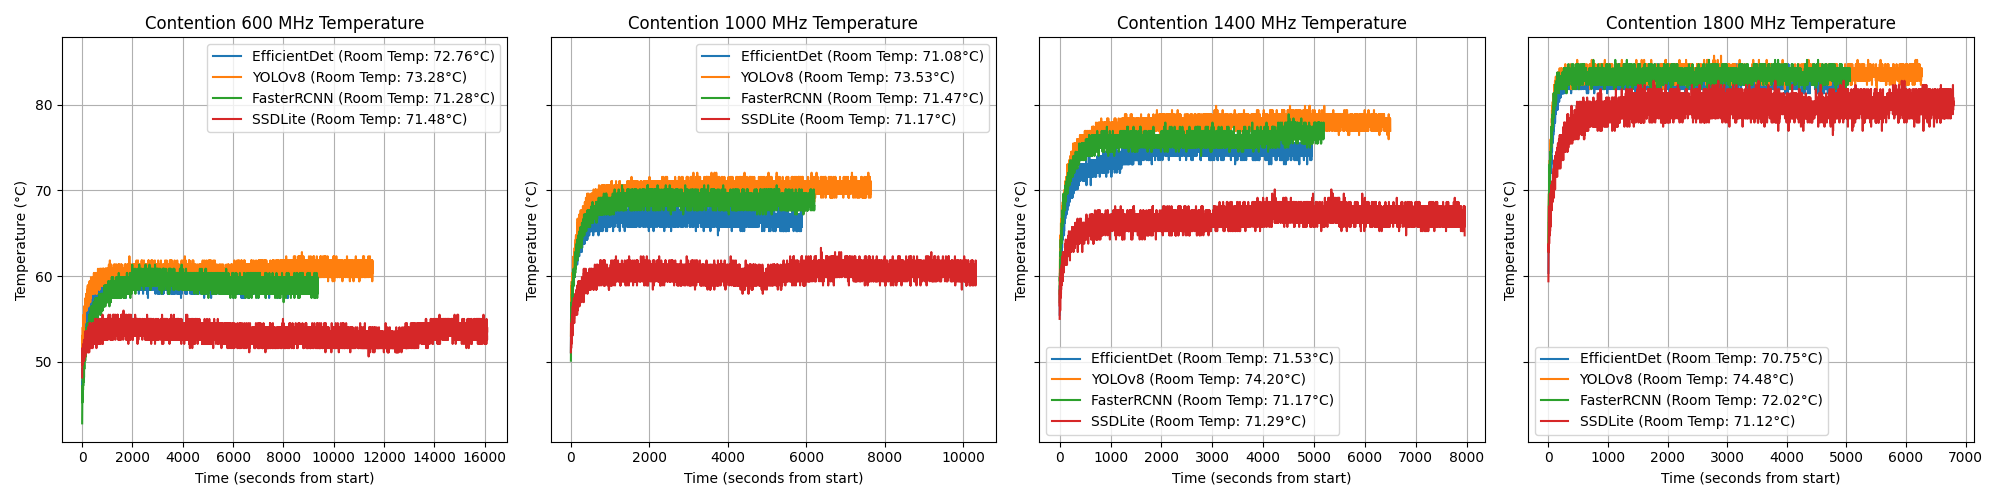
\includegraphics[width=1\linewidth]{images/temperature_plot.png}
  \caption{Temperature profiles of object detection models under various contention scenarios.}
  \label{fig:temperature_profiles}
\end{figure*}

\begin{figure*}[t]
  \centering
  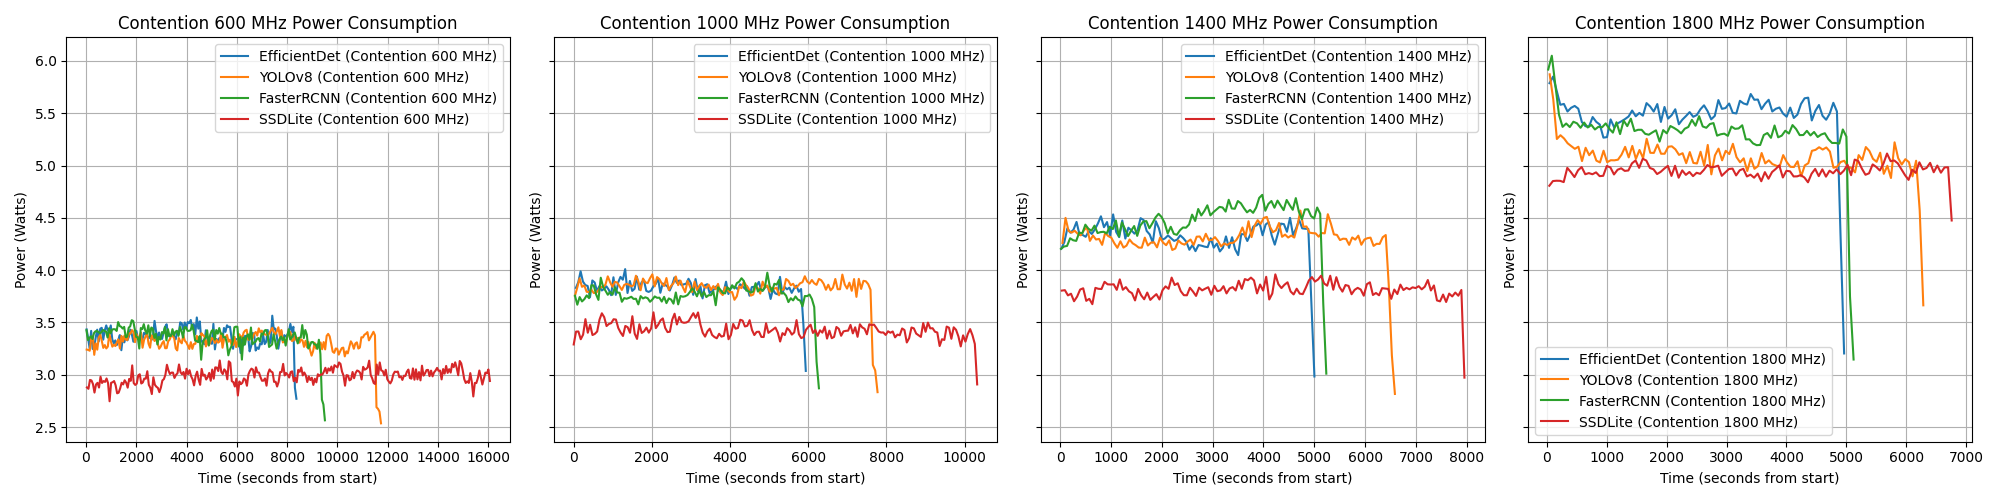
\includegraphics[width=1\linewidth]{images/power_consumption.png}
  \caption{Power consumption of object detection models across different CPU clock speeds.}
  \label{fig:power_consumption}
\end{figure*}

\begin{figure*}[t]
  \centering
  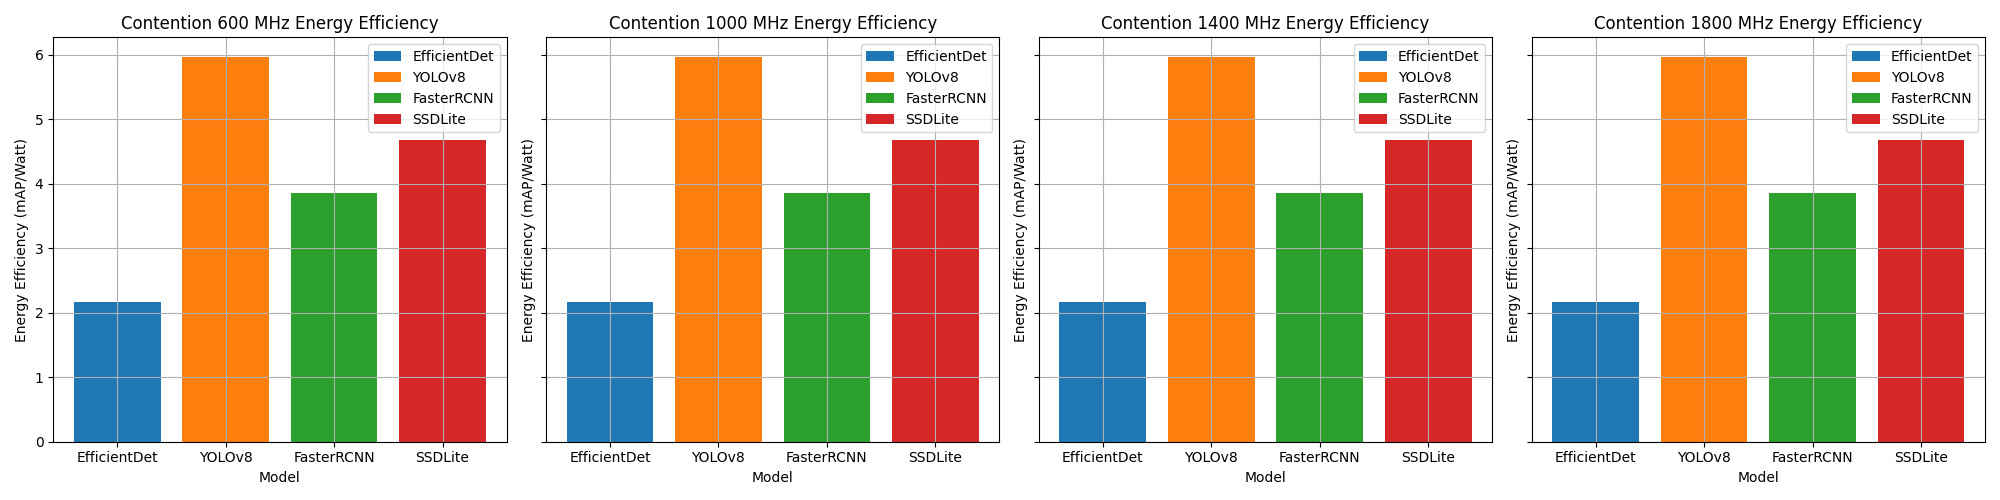
\includegraphics[width=1\linewidth]{images/energy_efficiency.png}
  \caption{Energy efficiency of object detection models, quantified as mAP per watt.}
  \label{fig:energy_efficiency}
\end{figure*}

\begin{figure*}[t]
  \centering
  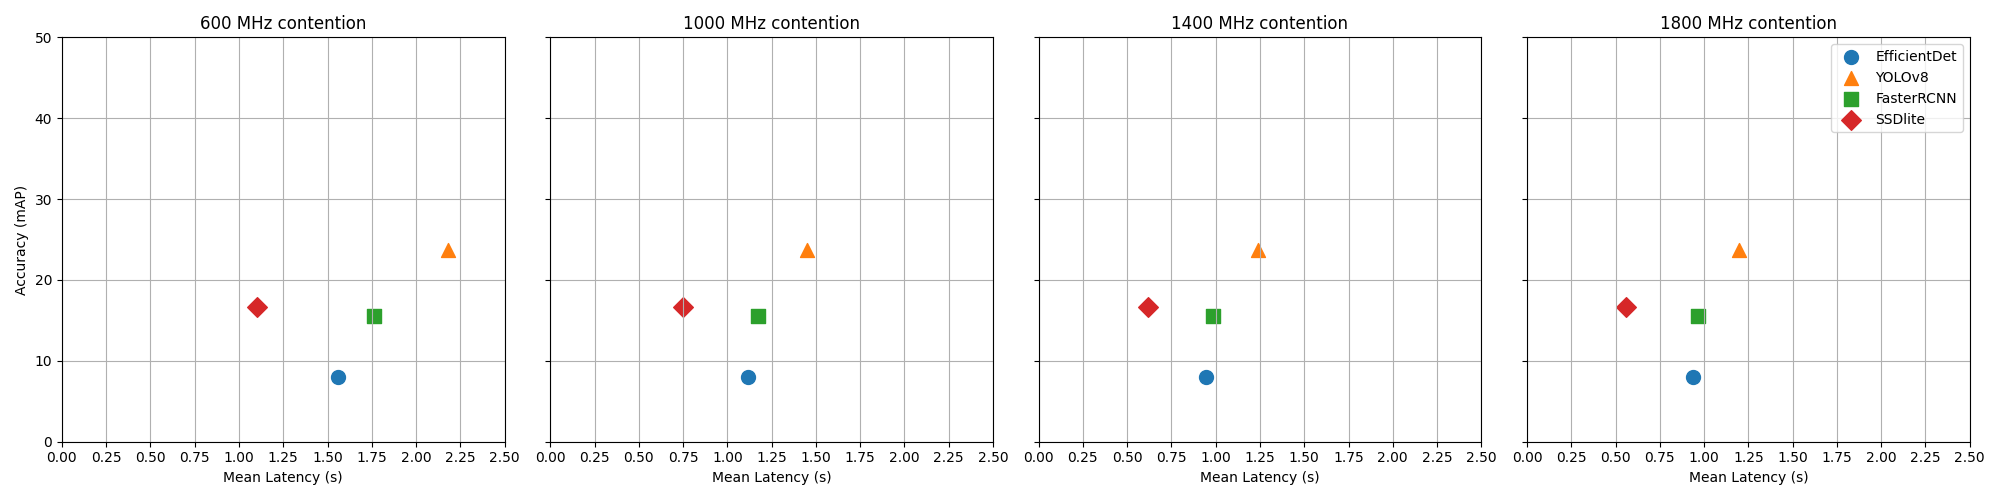
\includegraphics[width=1\linewidth]{images/accuracy_latency_graph.png}
  \caption{Comparison of accuracy (mAP) against mean latency for each object detection model.}
  \label{fig:accuracy_latency}
\end{figure*}

\begin{table*}[t]
\centering
\caption{Performance Metrics for Object Detection Models}
\label{tab:metrics}
\begin{tabular}{@{}lrrrrrrrr@{}}
Model & Latency (s) & FPS & mAP& AP50 & AP75 & AP\_small & AP\_medium & AP\_large \\
\midrule
YOLOv8 & 2.178 & 0.46 & 0.237 & 0.308 & 0.264 & 0.067 & 0.257 & 0.370 \\
YOLOv8 & 1.451 & 0.69 & 0.237 & 0.308 & 0.264 & 0.067 & 0.257 & 0.370 \\
YOLOv8 & 1.237 & 0.81 & 0.237 & 0.308 & 0.264 & 0.067 & 0.257 & 0.370 \\
YOLOv8 & 1.196 & 0.84 & 0.237 & 0.308 & 0.264 & 0.067 & 0.257 & 0.370 \\
\hline
SSDLite & 1.099 & 0.91 & 0.166 & 0.242 & 0.185 & 0.001 & 0.114 & 0.384 \\
SSDLite & 0.750 & 1.33 & 0.166 & 0.242 & 0.185 & 0.001 & 0.114 & 0.384 \\
SSDLite & 0.615 & 1.62 & 0.166 & 0.242 & 0.185 & 0.001 & 0.114 & 0.384 \\
SSDLite & 0.561 & 1.78 & 0.166 & 0.242 & 0.185 & 0.001 & 0.114 & 0.384 \\
\hline
FasterRCNN & 1.763 & 0.57 & 0.155 & 0.221 & 0.176 & 0.008 & 0.117 & 0.332 \\
FasterRCNN & 1.175 & 0.85 & 0.155 & 0.221 & 0.176 & 0.008 & 0.117 & 0.332 \\
FasterRCNN & 0.987 & 1.01 & 0.155 & 0.221 & 0.176 & 0.008 & 0.117 & 0.332 \\
FasterRCNN & 0.965 & 1.04 & 0.155 & 0.221 & 0.176 & 0.008 & 0.117 & 0.332 \\
\hline
EfficientDet & 1.560 & 0.64 & 0.080 & 0.100 & 0.092 & 0.001 & 0.048 & 0.169 \\
EfficientDet & 1.117 & 0.90 & 0.080 & 0.100 & 0.092 & 0.001 & 0.048 & 0.169 \\
EfficientDet & 0.943 & 1.06 & 0.080 & 0.100 & 0.092 & 0.001 & 0.048 & 0.169 \\
EfficientDet & 0.940 & 1.06 & 0.080 & 0.100 & 0.092 & 0.001 & 0.048 & 0.169 \\
\end{tabular}
\end{table*}



\end{document}
